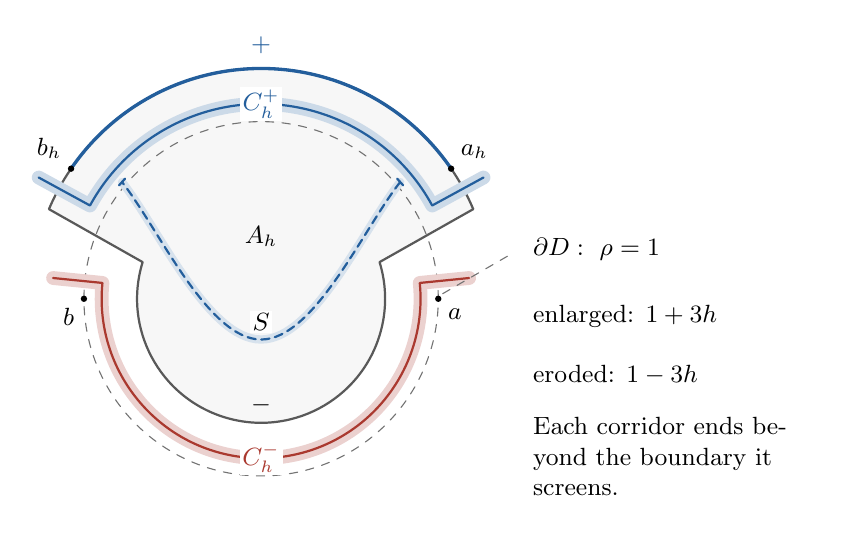
\begin{tikzpicture}[scale=2.25,line cap=round,line join=round,
  every node/.style={font=\small}]
 \definecolor{curveplus}{RGB}{35,94,156}
 \definecolor{curveminus}{RGB}{170,57,47}
 \fill[black!3]
   (17.2:.70)--(22.9:1.30) arc[start angle=22.9,end angle=157.1,radius=1.30]
   --(162.8:.70) arc[start angle=162.8,end angle=377.2,radius=.70]--cycle;
 \draw[black!65,thick]
   (17.2:.70)--(22.9:1.30) arc[start angle=22.9,end angle=157.1,radius=1.30]
   --(162.8:.70) arc[start angle=162.8,end angle=377.2,radius=.70];
 \draw[curveplus,very thick]
   (34.4:1.30) arc[start angle=34.4,end angle=145.6,radius=1.30];
 \draw[dashed,black!55] (0,0) circle[radius=1];
 \draw[curveminus!23,line width=5pt]
   (174.3:1.18)--(174.3:.90)
   arc[start angle=174.3,end angle=365.7,radius=.90]--(5.7:1.18);
 \draw[curveminus,thick]
   (174.3:1.18)--(174.3:.90)
   arc[start angle=174.3,end angle=365.7,radius=.90]--(5.7:1.18);
 \draw[curveplus!23,line width=5pt]
   (28.6:1.43)--(28.6:1.10)
   arc[start angle=28.6,end angle=151.4,radius=1.10]--(151.4:1.43);
 \draw[curveplus,thick]
   (28.6:1.43)--(28.6:1.10)
   arc[start angle=28.6,end angle=151.4,radius=1.10]--(151.4:1.43);
 \draw[curveplus!18,line width=3pt]
   (40:1.025) .. controls (.58,.40) and (.30,-.23) .. (0,-.23)
   .. controls (-.30,-.23) and (-.58,.40) .. (140:1.025);
 \draw[curveplus,densely dashed,thick]
   (40:1.025) .. controls (.58,.40) and (.30,-.23) .. (0,-.23)
   .. controls (-.30,-.23) and (-.58,.40) .. (140:1.025);
 \draw[curveplus,thick] (.768,.678)--(.802,.640);
 \draw[curveplus,thick] (-.768,.678)--(-.802,.640);
 \node[fill=white,inner sep=1pt] at (0,-.13) {$S$};
 \fill (0:1) circle[radius=.018] node[below right] {$a$};
 \fill (180:1) circle[radius=.018] node[below left] {$b$};
 \fill (34.4:1.30) circle[radius=.018] node[above right] {$a_h$};
 \fill (145.6:1.30) circle[radius=.018] node[above left] {$b_h$};
 \node at (0,.35) {$A_h$};
 \node[curveplus,fill=white,inner sep=1pt] at (0,1.10) {$C_h^+$};
 \node[curveminus,fill=white,inner sep=1pt] at (0,-.90) {$C_h^-$};
 \node at (0,-.60) {$-$};
 \node[curveplus] at (0,1.43) {$+$};
 \node[anchor=west] at (1.48,.28) {$\partial D:\ \rho=1$};
 \draw[dashed,black!55] (1.39,.24)--(1.01,.02);
 \node[anchor=west] at (1.48,-.10) {enlarged: $1+3h$};
 \node[anchor=west] at (1.48,-.43) {eroded: $1-3h$};
 \node[anchor=west,align=left,text width=3.7cm] at (1.48,-.89)
   {Each corridor ends beyond the boundary it screens.};
\end{tikzpicture}
